\begin{mainquestion}{thevenin_meas}{Measuring Thévenin}
A black box filled with linear circuitry is connected to a variable resistor.  An ideal ammeter (with zero resistance) and an ideal voltmeter (with infinite resistance) are used to measure current and voltage as shown below. The results of several sample readings are listed in the accompanying table.

\begin{table}[htbp]
\centering
\label{tab:measurements}
\begin{tabular}{|c | c |  c|}
\hline
\textbf{R ($\Omega$)} & \textbf{V (volts)} & \textbf{I (amps)} \\
\hline
4 &  & 1.5 \\ \hline
6 & 8 & \\ \hline
 & 9.6 & 1.2 \\ \hline
10 &  & 1 \\ \hline

\end{tabular}
\end{table}

\begin{partquestion}{missingdata}{Based on what you see in the table, fill in the missing values.}
\begin{answer}
Using Ohm's Law, $V=IR$ and we can determine the missing values:
\begin{table}[htbp]
\centering
\label{tab:measurementsfilled}
\begin{tabular}{|c | c |  c|}
\hline
\textbf{R ($\Omega$)} & \textbf{V (volts)} & \textbf{I (amps)} \\
\hline
4 & 6 & 1.5 \\ \hline
6 & 8 & 1.333\\ \hline
8 & 9.6 & 1.2 \\ \hline
10 & 10  & 1 \\ \hline
\end{tabular}
\end{table}
\end{answer}
\end{partquestion}

\begin{partquestion}{suspiciousdata}{It appears there is some suspicious data in the above table. Plot an estimate of the load line.  Can you determine which data row is wrong?  How do you know?}
\begin{answer}
For any linear system, plotting these data points on an I-V curve should result in a straight line.
\begin{center}
    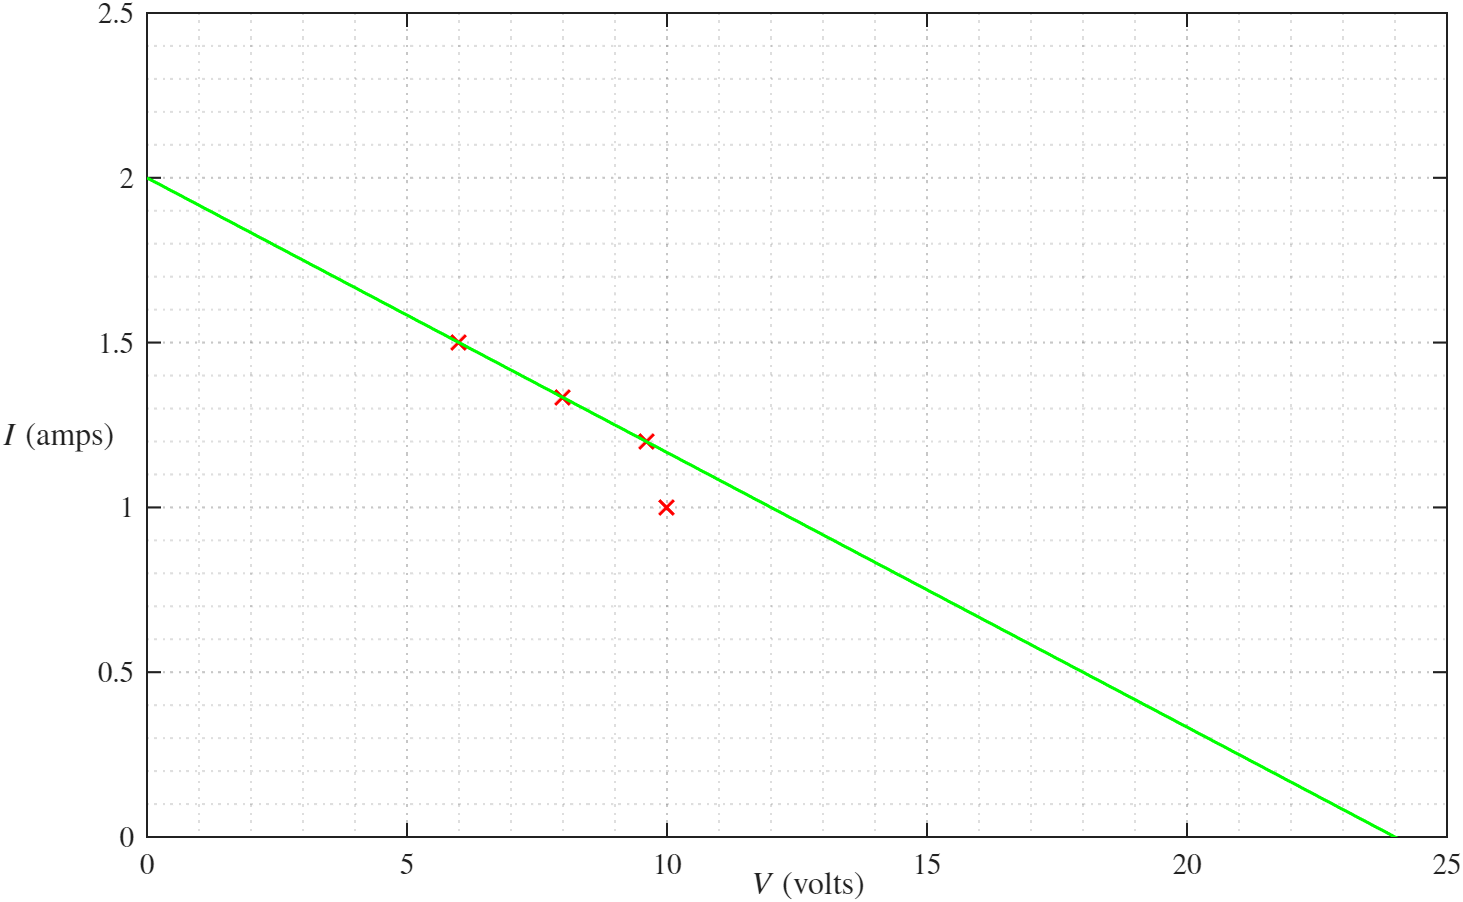
\includegraphics[width=4in]{figure.png}
\end{center}
We can see that there is one data point which is not co-linear with the other three; this point at (10 V, 1 A) must be invalid data.
\end{answer}
\end{partquestion}
\begin{partquestion}{iandv}{Find $I$ and $V$ when $R=\qty{17}{\ohm}$.}
\begin{answer}
Replace the black box by its Th\'evenin equivalent, consisting of a source $V_{\mathrm{th}}$ in series with a resistance $R_{\mathrm{th}}$. For a load
  resistance $R$,
  \[
    \frac{V}{V_{\mathrm{th}}}=\frac{R}{R+R_{\mathrm{th}}}.
  \]
  Using the measurements for $R=\qty{4}{\ohm}$ and $R=\qty{6}{\ohm}$ gives
  \[
    \frac{6}{V_{\mathrm{th}}}=\frac{4}{4+R_{\mathrm{th}}},
    \qquad
    \frac{8}{V_{\mathrm{th}}}=\frac{6}{6+R_{\mathrm{th}}}.
  \]
  Eliminating $V_{\mathrm{th}}$,
  \begin{align*}
    \frac{6}{4}(4+R_{\mathrm{th}})
      &= \frac{8}{6}(6+R_{\mathrm{th}}),\\
    6+\frac{3}{2}R_{\mathrm{th}}
      &= 8+\frac{4}{3}R_{\mathrm{th}},\\
    R_{\mathrm{th}} &= \qty{12}{\ohm}.
  \end{align*}
  It follows that
  \[
    V_{\mathrm{th}}
      =\frac{6}{4}(4+12)
      =\qty{24}{\volt}.
  \]
  Therefore, with $R=\qty{17}{\ohm}$,
  \[
    V=V_{\mathrm{th}}\frac{R}{R+R_{\mathrm{th}}}
      =24\frac{17}{17+12}
      =\frac{408}{29}\,\mathrm{V}
      \approx \qty{14.1}{\volt},
  \]
  and
  \[
    I=\frac{V}{R}
      =\frac{24}{29}\,\mathrm{A}
      \approx \qty{0.83}{\ampere}.
  \]
\end{answer}
\end{partquestion}
\begin{partquestion}{equation}{With your results from (\cref{prob:thevenin_meas:iandv}), now determine the exact equation for the load line sketched in (\cref{prob:thevenin_meas:suspiciousdata}) }
\begin{answer}
The equation is:
\[
    I=-\frac{V}{R_\mathrm{th}}+\frac{V_\mathrm{th}}{R_\mathrm{th}}
      =-\frac{V}{12}+2
  \]
\end{answer}
\end{partquestion}
\begin{partquestion}{rload}{Determine the value of $R$ that achieves maximum power transfer from the black box to the variable resistor.}
\begin{answer}
Maximum power transfer occurs when the load resistance equals the Th\'evenin
  resistance:
  \[
    \boxed{R=R_{\mathrm{th}}=\qty{12}{\ohm}.}
  \]
\end{answer}
\end{partquestion}
\begin{partquestion}{maxpower}{What is the maximum power transferred to the variable resistor?}
\begin{answer}
 With $R=R_{\mathrm{th}}$, the maximum load power is
  \[
    P_{\max}=\frac{V_{\mathrm{th}}^2}{4R_{\mathrm{th}}}
      =\frac{(\qty{24}{\volt})^2}{4(\qty{12}{\ohm})}
      =\boxed{\qty{12}{\watt}}.
  \]
\end{answer}
\end{partquestion}

\end{mainquestion}